\setchapterpreamble[ur][.6\textwidth]{%
\dictum[Fyodor Dostoyevsky, \textit{The Idiot} (1868--9)]{%
One can't understand everything at once, we can't begin with perfection all at once! In order to reach perfection one must begin by being ignorant of a great deal. And if we understand things too quickly, perhaps we shan't understand them thoroughly.}\vskip1em

\dictum[dude]{%
things}\vskip1em}

\chapter[Chapter 1: General introduction]{General introduction}
\chaptermark{General introduction}
%%%%%%%%%%%%%%%%%%%%%%%%%%%%%%%%%%%%%%%%%%%%%%%%%%%%%%%%%%%%%%%%%%%%%%%%%%%%%%%%%%%%%%

%%%%%%%%%%%%%%%%%%%%%%%%%%%%%%%%%%%%%%%%%%%
\section{Variation in fitness}
%variation in evolution
Understanding variation among living things is the heart of evolutionary questioning.


Darwin great discovery was to recognize the variation within species as the fuel generating the astonishing diversity of species themselves.

%fitness
There has been a great deal written about the concept of fitness, and as is common for central scientific concepts REF?, its definition is problematic. Actually, there are many definitions, and sub-definitions. 
In this thesis, what we mean by \emph{fitness} is ...
most adapted to the study framework.
with the difficulty that... 


In this thesis, we will not really deal with the fundamental question of appearance and maintenance of variation in fitness (e.g. lek paradox, see XX), but rather with its proximal sources.

 
%%%%%%%%%%%%%%%%%%%%%%%%%%%%%%%%%%%%%%%%%%%
\section{Quantitative genetics}

How to measure and make sense of genetic variation?
For over a century, there have been two main approaches. 
These can be summarized as ``bottom-up'' and ``top-down''.
The Mendelians and the biometricians



intronic region of the fat metabolism and food intake-related \emph{lepr} gene

We found a recessive allele (let call the recessive allele \emph{a}, and the dominant allele \emph{A}) associated with lighter individuals (Fig. \ref{fig:leprpheno}). Homozygotes \emph{aa} were -2.9 g lighter (95\% credibility interval $[0.6;5.1]$), that is, 8\% lighter than the mean. 


\begin{figure}[ht]
	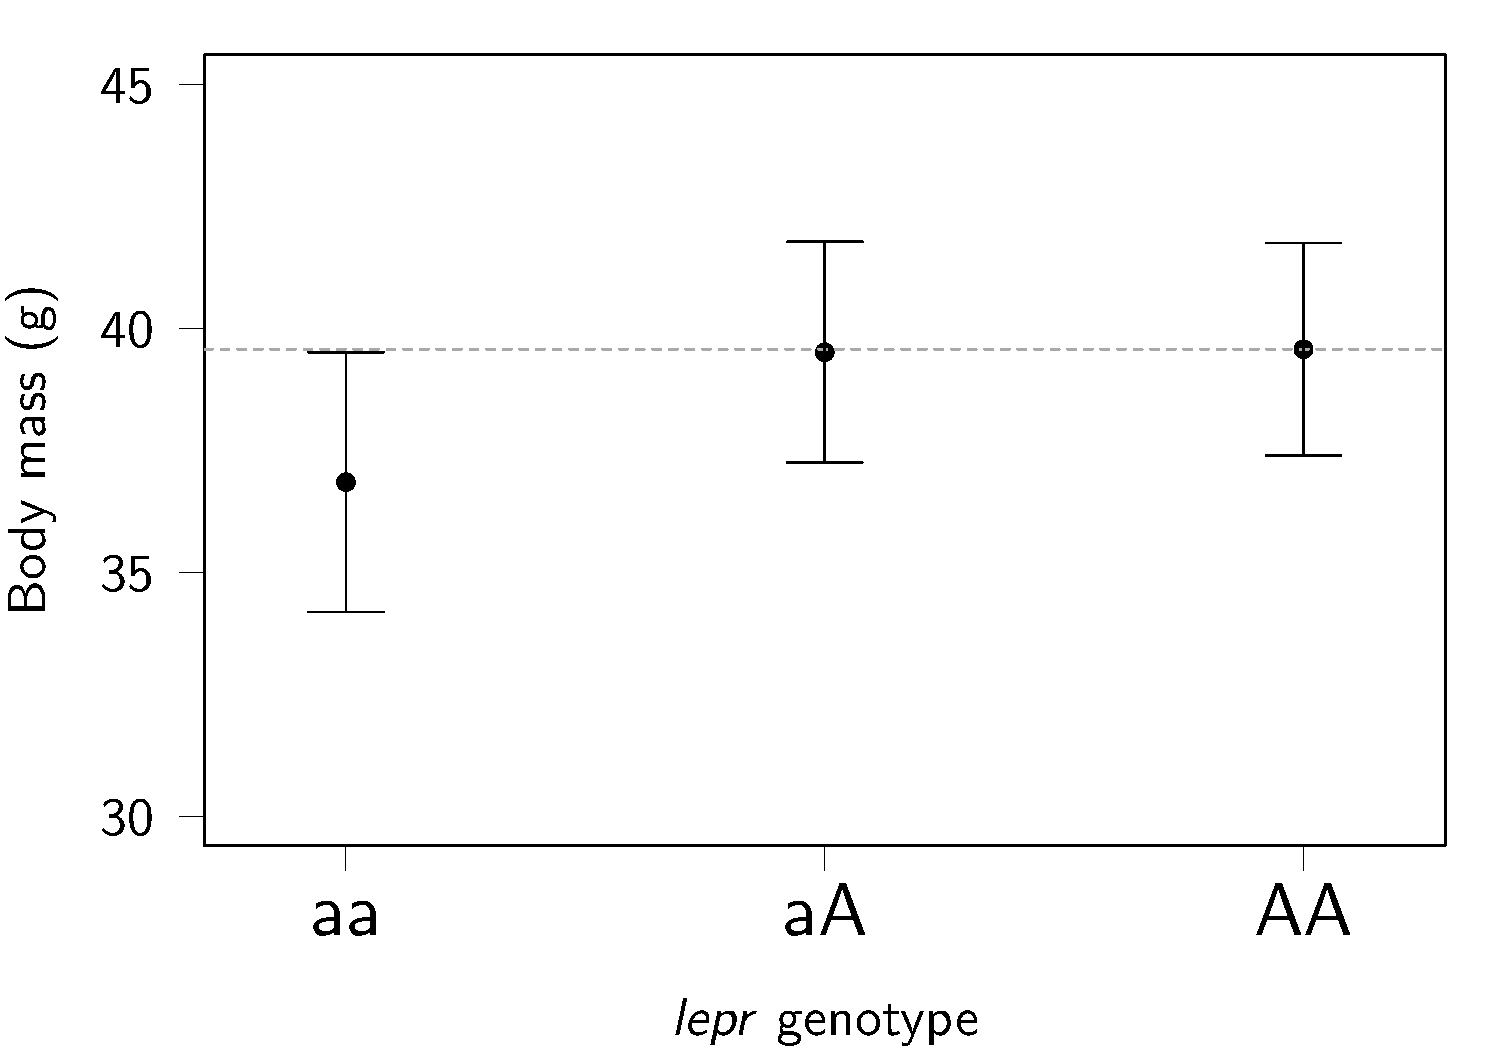
\includegraphics[width=1\textwidth]{FiguresGeneral/PhenoEffect-1}
	\caption{Expected body mass of snow voles bearing the three \emph{lepr} genotypes. The expectations and 95\% confidence intervals were predicted from a linear mixed model fitted to the 2311 mass measurement of 532 snow voles. The model accounted for sex, age, date of capture and their two-ways interactions, as well as year of capture and multiple measurements of the same individual.}
	\label{fig:leprpheno}
\end{figure}

Despite such a dramatic effect, \emph{lepr} genotypic variation explains only 1.3\% of the additive genetic variation estimated from an animal model. This proportion can seem small, but in particular because the homozygotes \emph{aa} are rare (3\% of all individuals genotyped).

Could we not simply sequence many more genes to explain a larger proportion of genetic variation?
The uncertainty in the estimation of the effect of \emph{lepr} translates into a Bayesian p-value of $0.01$. 
If other genetic loci were analysed, 


%%%%%%%%%%%%%%%%%%%%%%%%%%%%%%%%%%%%%%%%%%%
\section{This thesis}

\subsection{Objectives}

\subsection{Churwalden snow voles}

\subsection{Thesis outline}


